%!TEX root = paper.tex
\section{Example}
Consider the hierarchical network in \Cref{fig:example} which
is split into three OSPF domains, and these domains communicate
using BGP. Host A talks to host B and C with the following policies:
traffic to B must go through a firewall at router $R_5$ and traffic 
to B and C do not share any links (We discuss the policy support in
detail in \Cref{sec:policy}). Given the particular domain assignment, 
we have to synthesize OSPF and BGP configurations satisfying the 
following policies. Illustrating our two-phase approach, we first 
use Genesis to find policy-compliant paths (indicated by the blue and
red paths). Note that there exists multiple solutions for the given
policies, we show how the control plane is 
synthesized using one of the solutions:
\begin{figure}
	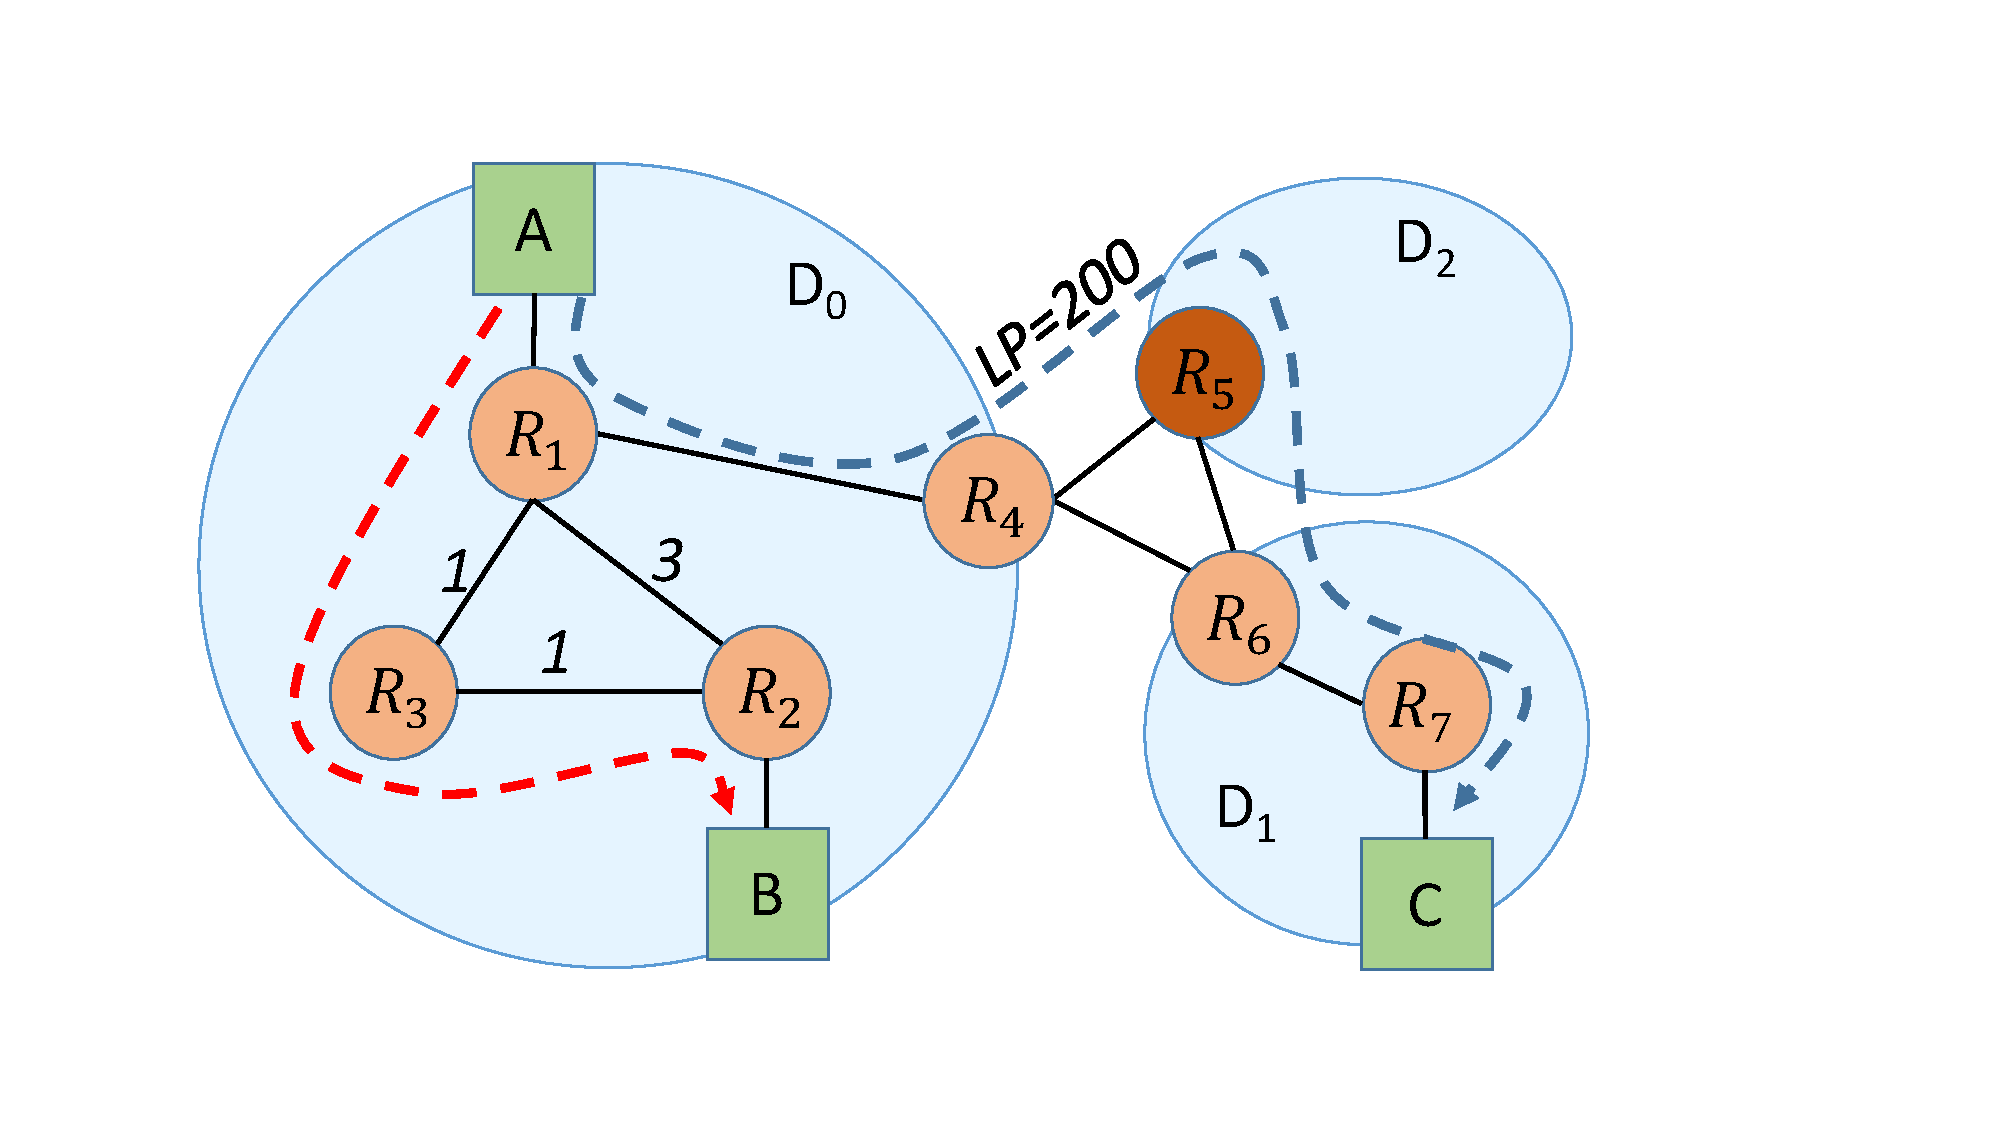
\includegraphics[width=0.75\columnwidth]{figures/example.pdf}
	\compactcaption{Example demonstrating the two-phase synthesis approach. 
	Genesis produces policy-compliant paths (red and blue), 
	which are used as input by Zeppelin to
	synthesize the OSPF and BGP configurations.}
	\label{fig:example}
\end{figure}

\begin{itemize}
	\item
For traffic $A \rightarrow B$, the path is entirely inside
a single OSPF domain, so Zeppelin has to find OSPF weights 
such that the shortest path is $R_1 \rightarrow R_3 \rightarrow 
R_2$. From the OSPF weights shown in \Cref{fig:example}, 
we can see that the weight of path $R_1 
\rightarrow R_3 \rightarrow R_2$ (2) is smaller than that of path
$R_1 \rightarrow R_2$ (3). 
 	\item For traffic $A \rightarrow C$, the path traverses through 
 	multiple domains, so Zeppelin configures BGP such that 
 	routing across domains follows the Genesis path. In this case, 
 	we need traffic to go through a longer path in terms of AS path
 	length; Zeppelin sets $R_4$'s BGP local preference for route C
 	from $R_5$ a higher value (200), so that $R_5$ is 
 	preferred over $R_6$. 
 	\item Suppose the operator wanted to compute a better domain
 	assignment for the network. We can see that if $R_5$ was moved
 	to $D_1$, we do not need to configure the local preference 
 	at $R_4$ as $R_5$ will be on the shortest AS path, 
 	thus, simplifying the BGP configuration. 
 	Zeppelin can find better domain assignments using a stochastic
 	search procedure. 
\end{itemize}